\documentclass[9pt,a4paper,landscape]{article}

\usepackage[left=1.50cm, right=1.50cm, top=1.50cm, bottom=1.50cm]{geometry}
\usepackage{amsmath}
\usepackage{amsfonts}
\usepackage{amssymb}
\usepackage{graphicx}
\usepackage{longtable}
\usepackage{booktabs}
\usepackage{lipsum}
\usepackage{multirow}
\usepackage{array}
\usepackage{ulem}
\usepackage{titlesec}
\usepackage{enumitem}
\usepackage{xcolor}
\usepackage{forest}



\newcolumntype{L}{>{\raggedright\arraybackslash}p{2.5cm}}
\newcolumntype{X}{>{\raggedright\arraybackslash}p{4cm}}

\titleformat*{\section}{\normalsize\bfseries}
\titleformat*{\subsection}{\normalsize\bfseries}

\newcommand{\msout}[1]{\text{\sout{$#1$}}}

\newcommand{\ngtb}[1]{T_{ \{#1\} }}
\newcommand{\ngfb}[1]{F_{ \{#1\} }}
\newcommand{\ngta}[1]{T_{#1}}
\newcommand{\ngfa}[1]{F_{#1}}

%An atom that must be true is formatted like $\ngta{}$, a body that must be true $\ngtb{}$, an atom that must be false, like $\ngfa{}$, and a body that must be false $\ngfb{}$.

\setlength\parindent{0pt}

\begin{document}
	
% ----------------------------------------------------------------------
	
{\small
	
\textbf{Cheatsheet for Answer Set Programming} \hfill Elizabeth Pankratz, WS 2019/20
	
\section{Algorithms and walk-throughs}

\vspace{\baselineskip}

% ----------------------------------------------------------------------

\subsection{Tips for determining stable models of normal programs}

If there are no obvious starting points for solving a program, i.e.\ no facts, unjustifiable atoms (those not appearing in heads of rules), or choice rules or even loops through negation (i.e.\ $1\{a, b\}1$ or $\{a \leftarrow {\sim} b, b \leftarrow {\sim} a\}$), then start by \textbf{assuming that the heads of negative rules are true} and looking for what that implies.\\

Also, if there are variables involved, then \textbf{assuming that a negated body atom really is false} often provides a good starting point.

\vspace{\baselineskip}

% ----------------------------------------------------------------------

\subsection{Computing the reduct}
\label{subsec:reduct}

To compute the reduct $P^X$ wrt a set of atoms $X$ for a program $P$:

\begin{enumerate}[noitemsep]
	\item Remove all rules in $P$ whose bodies contain one or more negative atoms whose positive counterparts are contained in $X$.
	\item Then, remove any remaining negative atoms whose positive counterparts were not contained in $X$, but leave the rest of the rule intact.
\end{enumerate}

\noindent This remaining set of positive rules is your reduct $P^X$.
Then, to determine the consequence of the reduct $Cn(P^X)$, create a set out of only those atoms which are justified by the remaining rules ( $Cn(P^X)$ = the ``transitive closure'' or ``minimal model of the reduct'').
If this closure matches the input set $X$, then $X$ is a stable model of $P$.\\

\noindent Let's see this in action for the program $P$ = \texttt{b :- not a. a :- not b.} and the set $X$ = \texttt{\{ a \}}.

\begin{center}
	\begin{tabular}{p{5cm}p{5cm}}
		Step & Reduct-in-progress \\ \midrule
		
		0 (original program)	& \texttt{b :- not a. \newline a :- not b.} \\&\\
		
		1 (remove rules where any atom in $X$ is negative) & \texttt{\sout{b :- not a.} \newline a :- not b.} \\&\\
		
		2 (remove all remaining negative atoms)	& \texttt{\sout{b :- not a.} \newline a :- \sout{not b.}} \\&\\
		
		$P^X$ & \texttt{a :- .}
	\end{tabular}
\end{center}

\noindent The consequence of this stable model is $Cn(P^X) =$ \texttt{\{ a \}}.
Because what went in, $X$, is the same as what came out, $Cn(P^X)$, we know that \texttt{\{ a \}} is a stable model of $P$.

%\begin{tabular}{lllll}
%	content...
%\end{tabular}

\pagebreak

% ----------------------------------------------------------------------

\subsection{Computing the Clark's Completion and getting its supported models}
\label{subsec:compl-supp}

Given a program $P$, compute the completion $CF(P)$ as follows.

\begin{enumerate}[noitemsep]
	\item Begin by writing down every atom in the program followed by $\leftrightarrow$ on a new line.
	\item Then, for each atom, find the rules with that atom in the head in $P$.
	\begin{enumerate}[noitemsep]
		\item If there is only one, then write its body to the right of the $\leftrightarrow$ (using logical negation).
		\item If there is more than one rule, create a disjunction out of all of the possible bodies and write this disjunction to the right of $\leftrightarrow$ (using logical negation and disjunction).
		\item If there is a fact for this atom, write $\top$.
		\item If there is no justification for this atom, write $\bot$.
	\end{enumerate}
\end{enumerate}

For example, given the program $P = \left\{\begin{array}{l}
a \leftarrow b \\
a \leftarrow {\sim} c \\
b \leftarrow d\\
d \leftarrow 
\end{array}\right\}$:

\begin{center}
	\begin{tabular}{p{3cm}p{5cm}}
		Step & Completion-in-progress\\ \midrule
		1 (set-up) & 	$CF(P) = \left\{\begin{array}{l}
		a \leftrightarrow  \\
		b \leftrightarrow  \\
		c \leftrightarrow  \\
		d \leftrightarrow 
		\end{array}\right\}$ \\ &\\
		%
		2a (one rule) & 	$CF(P) = \left\{\begin{array}{l}
		a \leftrightarrow  \\
		b \leftrightarrow d \\
		c \leftrightarrow  \\
		d \leftrightarrow 
		\end{array}\right\}$ \\ &\\
		%
		2b (multiple rules) & 	$CF(P) = \left\{\begin{array}{l}
		a \leftrightarrow b \lor (\neg c) \\
		b \leftrightarrow d \\
		c \leftrightarrow  \\
		d \leftrightarrow 
		\end{array}\right\}$ \\ &\\
		%
		2c (facts) & 	$CF(P) = \left\{\begin{array}{l}
		a \leftrightarrow b \lor (\neg c) \\
		b \leftrightarrow d \\
		c \leftrightarrow  \\
		d \leftrightarrow \top
		\end{array}\right\}$ \\ &\\
		%
		2d (no justifcation) & 	$CF(P) = \left\{\begin{array}{l}
		a \leftrightarrow b \lor (\neg c) \\
		b \leftrightarrow d \\
		c \leftrightarrow \bot \\
		d \leftrightarrow \top
		\end{array}\right\}$ \\
	\end{tabular}
\end{center}

To find the \textbf{supported model of the completion}: if the completion contains $\top$s or $\bot$s, start with those, seeing what they imply.
Write out everything you know from the completion (i.e.\ positive and negative atoms), adding to this set iteratively as the known atoms imply others, and then take the positive atoms as the supported model.
For the above example:
\vspace{-.5\baselineskip}
\begin{center}
	$\{d, \neg c\} \rightarrow \{d, \neg c, b\} \rightarrow \{d, \neg c, b, a\} = \{a, b, d\}$
\end{center}
\vspace{-.5\baselineskip}
Can also look for odd loops through negation (i.e.\ something like $\{ d \leftrightarrow \neg e, \hspace{3pt}  e \leftrightarrow \neg d \}$, which starts you off with the beginnings of two supported models, one containing $\{d, \neg e\}$ and one $\{e, \neg d\}$). If nothing else, assume one atom and use trial-and-error. If the program contains a loop, there will be one supported model with the loop atoms and one without.

\pagebreak

% ----------------------------------------------------------------------

\subsection{Computing loop formulas}
\label{subsec:lf}

Given a program $P$ that contains a set of loops $loops(P)$ (which are most easily found visually using a dependency graph; see glossary), compute the loop formulas $LF(P)$ (= formulas that forbid a loop from being in a stable model) as follows.

\begin{enumerate}[noitemsep]
	\item Begin by writing out the disjunction of all atoms involved in each loop, followed by $\rightarrow$, on a new line.
	\item Using the original program (not the completion):
	\begin{enumerate}[noitemsep]
		\item Identify all rules whose heads contain an atom involved in the loop.
		\item Disqualify any rules if their positive body contains any of the atoms involved in the loop.
		\item Take the bodies of the remaining rules and form a disjunction out of them, writing this to the right of $\rightarrow$.
	\end{enumerate}
\end{enumerate}

For example, for the program $P = \left\{\begin{array}{lll}
a \leftarrow & b \leftarrow {\sim} a & b \leftarrow c, d\\
c \leftarrow a, {\sim} e & d \leftarrow b, c & d \leftarrow e, {\sim} a\\
\end{array}\right\}$, which contains $loops(P) = \{ \{b, d\} \}$:

\begin{center}
	\begin{tabular}{p{3cm}p{5cm}p{6cm}}
		Step & Loop-formula-in-progress & Rules \\ \midrule
		1 (set-up) & $b \lor d \rightarrow$ & \\ & \\
		%
		2a (identify rules) &  & $\begin{array}{l}
		b \leftarrow {\sim} a\\
		d \leftarrow b, c\\
		b \leftarrow c, d\\
		d \leftarrow e, {\sim} a
		\end{array}$  \\ & \\
		%
		2b (disqualify rules) &  & $\begin{array}{ll}
		b \leftarrow {\sim} a & \checkmark \\
		\msout{d \leftarrow \underline{b}, c} & \times  \text{ (loop atom in pos body)}\\
		\msout{b \leftarrow c, \underline{d}} & \times  \text{ (loop atom in pos body)}\\
		d \leftarrow e, {\sim} a & \checkmark
		\end{array}$  \\ & \\
		%
		2c (disjunction) & $b \lor d \rightarrow (\neg a) \lor (e \land \neg a)$
	\end{tabular}
\end{center}

Loop formulas are written as a set: $LF(P) = \{ b \lor d \rightarrow (\neg a) \lor (e \land \neg a) \}$.
\vspace{\baselineskip}

% ----------------------------------------------------------------------

\subsection{Using loop formulas to identify stable models}

To see if a supported model is also a stable model, we can check if the supported model satisfies the implication in the loop formula.
If yes, then it is a stable model.

\vspace{\baselineskip}

Formally: stable models = $CF(P)\ \cup$ loop formulas.

\vspace{\baselineskip}

For the above example, the supported models of the completion are $\{a, c\}$ and $\{a, c, b, d\}$ (one with the loop atoms and one without).

\begin{center}
	\begin{tabular}{llp{20cm}}
		$\checkmark$ & $\{a, c\}$ & The precondition of the loop formula, $b \lor d$, is false, since neither $b$ nor $d$ is in the model. This makes the implication true. Thus $\{a, c\}$ is a stable model. \\
		$\times$ & $\{a, c, b, d\}$ & The precondition of the loop formula is true, since $b$ or $d$ is in the model (in fact, both are). However, the RHS is not fulfilled: we have $\neg e$ (by virtue of $e$ not being in the model) and $a$, while the implication requires $e$ and $\neg a$. Thus the loop formula is not satisfied, so $\{a, c, b, d\}$ is not a stable model.\\
	\end{tabular}
\end{center}

It is possible for none of the supported models to be stable models if no models satisfy the loop formulas. Then the program has no stable models.\\


If there are several loop formulas, a model only has to fail one of them to be disqualified from being a stable model (sudden death!).

\pagebreak

% ----------------------------------------------------------------------

\subsection{Finding the Greatest Unfounded Set and all unfounded sets}
\label{subsec:unf}

Find all unfounded sets of a program $P$ wrt a partial interpretation $\langle \{\top\}, \{\bot\} \rangle$ as follows:
\begin{enumerate}[noitemsep]
	\item Remove rules from the program that are incompatible with the partial interpretation (i.e.\ where an atom in the negative body is in $\{\top\}$, or where an atom in the positive body is in $\{\bot\}$).
	\item Compute the second step of the reduct for the remaining rules, crossing out all remaining negative atoms in bodies.
	\item Get the minimal model of the reduct (= those atoms that are justifiable using the remaining rules in the program).
	\item Take the complement of the minimal model wrt all atoms in the program, $A$. The result is the greatest unfounded set (GUS).
	\item Generate all subsets of the GUS and check to see if each of those is unfounded using the criteria below.
\end{enumerate}

Unfoundedness criteria: A set of atoms $U$ is unfounded wrt some partial interpretation if \textbf{all rules} in the program whose heads are atoms in $U$ meet at least one of the following conditions:

\begin{enumerate}[noitemsep, label=(\roman*)]
	\item one atom of the rule's positive body is false in the partial interpretation (i.e.\  $\langle \{\}, \{\text{atom}\} \rangle$)
	\item one atom of the rule's negative body is true in the partial interpretation (i.e.\  $\langle \{\text{atom}\}, \{\} \rangle$)
	\item one atom of the rule's positive body is also in $U$
\end{enumerate}

For example, given the program $P = \left\{\begin{array}{lll}
a \leftarrow {\sim} d & b \leftarrow {\sim} a & b \leftarrow d, e\\
c \leftarrow a, {\sim} e & d \leftarrow b, c & e \leftarrow d, {\sim} c\\
\end{array}\right\}$ and the partial interpretation $\langle \{a\}, \{b\} \rangle$:

\begin{center}
	\begin{tabular}{p{5cm}p{9cm}p{8cm}}
	Step & Work-in-progress & Notes\\ \midrule
	%
	1 (remove incompatible rules) & $P = \left\{\begin{array}{lll}
	a \leftarrow {\sim} d & \msout{b \leftarrow \underline{{\sim} a}} & b \leftarrow d, e\\
	c \leftarrow a, {\sim} e & \msout{d \leftarrow \underline{b}, c} & e \leftarrow d, {\sim} c\\
	\end{array}\right\}$ & $a$ is $\top$ but in neg body; $b$ is $\bot$ but in pos body. \\ &\\
	%
	2 (rm neg atoms to get reduct) & $P = \left\{\begin{array}{lll}
	a \leftarrow \msout{{\sim} d }& \msout{b \leftarrow {\sim} a} & b \leftarrow d, e\\
	c \leftarrow a, \msout{{\sim} e} & \msout{d \leftarrow b, c} & e \leftarrow d, \msout{{\sim} c}\\
	\end{array}\right\}$ & \\ &\\
	%
	3 (minimal model) & $\{a, c\}$ & (this doesn't necessarily mean that these atoms are actually true)\\ &\\
	%
	4 (complement wrt $A$) &  $A \backslash \{a, c\} = \{a, b, c, d, e\} \backslash \{a, c\} = \{b, d, e\}$ & Thus, the GUS is $\{b, d, e\}$. \\ &\\
	%
	5 (subsets unfounded?) & $\begin{array}{lllc} 
		\text{Subsets of GUS} & \text{Rules} & \text{Unf.\ criterion} & U \text{ unf?}\\ \midrule
		U = \{b, d\} 	& b \leftarrow \underline{{\sim} a} 	& (ii)\ a = \top & \\
						& b \leftarrow \underline{d}, e		& (iii)\ d \in U & \\
						& d \leftarrow \underline{b}, c		& (iii)\ b \in U, = \bot & \checkmark \\ \midrule
						%
		U = \{b, e\} 	& b \leftarrow \underline{{\sim} a} 	& (ii)\ a = \top & \\
						& b \leftarrow d, \underline{e}		& (iii)\ e \in U & \\
						& e \leftarrow d, {\sim} c			& \text{external support} & \times \\ \midrule
						%
		U = \{d, e\} 	& d \leftarrow \underline{b}, c 	& (i)\ b = \bot & \\
						& e \leftarrow \underline{d}, {\sim} c& (iii)\ d \in U & \checkmark \\ \midrule
						%
		U = \{b\} 		& b \leftarrow \underline{{\sim} a} 	& (ii)\ a = \top & \\
						& b \leftarrow d, e					& \text{external support} & \times \\ \midrule
						%
		U = \{d\} 		& d \leftarrow \underline{b}, c		& (iii)\ b = \bot & \checkmark \\ \midrule
						%
		U = \{e\} 		& e \leftarrow d, {\sim} c 			& \text{external support} & \times \\ \midrule
		U = \varnothing 	&  & & \checkmark \\ \midrule
	\end{array}$
	& Thus, the unfounded sets are $\{b, d, e\}$ (the GUS), $\{b,d\}, \{d,e\}, \{d\}$, and $\varnothing$. \\
\end{tabular}
\end{center}

\pagebreak

% ----------------------------------------------------------------------

\subsection{Using loop formulas on unfounded sets}
\label{subsec:lf-unf}

(Apparently we can do this. I don't know why or what good it does.)\\


Using the same method as outlined above for computing loop formulas for the elements of $loops(P)$, loop formulas can also be calculated for unfounded sets.
Then the formulas are compared to the partial interpretation used to generate the unfounded sets.\\


For example, using two of the unfounded sets identified above, $\varnothing$ and $\{b,d\}$, for the program $P = \left\{\begin{array}{lll}
a \leftarrow {\sim} d & b \leftarrow {\sim} a & b \leftarrow d, e\\
c \leftarrow a, {\sim} e & d \leftarrow b, c & e \leftarrow d, {\sim} c\\
\end{array}\right\}$ and the partial interpretation $\langle \{a\}, \{b\} \rangle$:

\begin{center}
	\begin{tabular}{p{3cm}p{5cm}p{6cm}}
		Step & Loop-formulas-in-progress & Rules \\ \midrule
%		1 (set-up) & $\varnothing \rightarrow$ & \\
		n/a (empty set) & $LF_P(\varnothing) = \{ \bot \rightarrow \bot \}$ & \\ \midrule
		
		1 (set-up) & $b \lor d \rightarrow$ & \\ & \\
		%
		2a (identify rules) &  & $\begin{array}{l}
		b \leftarrow {\sim} a\\
		b \leftarrow d, e\\
		d \leftarrow b, c
		\end{array}$  \\ & \\
		%
		2b (disqualify rules) &  & $\begin{array}{ll}
		b \leftarrow {\sim} a &  \\
		b \leftarrow \underline{d}, e & \times \hspace{8pt} (d \in U) \\
		d \leftarrow \underline{b}, c & \times \hspace{8pt} (b \in U) 
		\end{array}$  \\ & \\
		%
		2c (disjunction) & $LF_P( \{b, d\} ) = \{b \lor d \rightarrow \neg a\}$ \\ \midrule
	\end{tabular}
\end{center}

\pagebreak

% ----------------------------------------------------------------------

\subsection{Computing Fitting Semantics}
\label{subsec:fitting-sem}

A technique for iteratively constructing an interpretation of a program (equivalent to the completion, so resulting in a supported model).

\begin{enumerate}[noitemsep]
	\item Start with $\Phi^0 \langle \varnothing, \varnothing \rangle = \langle \varnothing, \varnothing \rangle$
	\item For $\Phi^1$, get facts and atoms with no rules and assign them to the appropriate set in the interpretation (i.e.\ true atoms to the set on the left, false atoms to the set on the right).
	\item For  $\Phi^n (n>1)$, use the current knowledge in the interpretation to figure out the truth value of further atoms.
	\item Eventually, either a fixpoint will be reached (the Least Fitting Fixpoint, excluding non-externally-supported loop atoms from the $\top$ set), or all of the atoms involved in the program will be assigned to a truth value in the interpretation. Either way, we can stop at that point, and the atoms that are $\top$ constitute the supported model.
\end{enumerate}

Stopping once all the atoms are collected is allowed because the Fitting operator is monotonic: can only add to it (as soon as you know an atom is true, it stays true).

For example, given the program $P = \left\{\begin{array}{lll}
a \leftarrow b, {\sim} e & b \leftarrow {\sim} c & c \leftarrow {\sim} a \\
a \leftarrow {\sim} d & c \leftarrow d, {\sim} e & d \leftarrow
\end{array}\right\}$, we calculate the Fitting Semantics as follows.

\begin{center}
	$\begin{array}{llll}
\text{Step} & \text{Fitting-in-progress} & \text{Rules} & \text{Notes} \\ \midrule
1 & \Phi^0 \langle \varnothing, \varnothing \rangle = \langle \varnothing, \varnothing \rangle && \\&\\
2 & \Phi^1 \langle \varnothing, \varnothing \rangle = \langle \{d\}, \{e\} \rangle & d \leftarrow & \text{no rule for}\ e, \text{so can call}\ \bot\\&\\
3 & \Phi^2 \langle \varnothing, \varnothing \rangle = \langle \{d, c\}, \{e\} \rangle & c \leftarrow d, {\sim} e & \text{only need one rule to call an atom}\ \top \\&\\
3 & \Phi^3 \langle \varnothing, \varnothing \rangle = \langle \{d, c\}, \{e, b\} \rangle & b \leftarrow {\sim} c & \text{no other rules to derive}\ b, \text{so can call}\ \bot \\&\\
3 & \Phi^4 \langle \varnothing, \varnothing \rangle = \langle \{d, c\}, \{e, b, a\} \rangle & \begin{array}{@{}l}
a \leftarrow b, {\sim} e\\
a \leftarrow {\sim} d
\end{array} & \text{neither rule is usable, so now can safely call}\ a\ \bot \\ &\\
4 & \text{total interpretation -- done}
\end{array}$
\end{center}

Therefore, the supported model of the above program is the true bit of the interpretation: $\{c, d\}$.
The resulting interpretation does not explicitly exclude the loop atoms without external support, which is why we need Wellfounded Semantics.

% ----------------------------------------------------------------------

\subsection{Computing Wellfounded Semantics}
\label{subsec:wellf-sem}

Similar to Fitting Semantics, except that, for the false set in the interpretation, we use the greatest unfounded set (GUS), rather than just using those atoms that can't be justified in the program in each iteration.
Loop atoms without any external support are contained in the GUS.

\begin{enumerate}[noitemsep]
	\item Start with $\Omega^0 \langle \varnothing, \varnothing \rangle = \langle \varnothing, \varnothing \rangle$
	\item For $\Omega^1$:
	\begin{enumerate}[noitemsep]
		\item $\top$ set: fill with facts from the program.
		\item $\bot$ set: compute the GUS wrt knowing that whatever atoms are in the $\top$ set so far are true (i.e.\ (1) remove rules containing negated atoms in the $\top$ set, (2) remove any remaining negated atoms, (3) compute the minimal model of this reduct, and (4) subtract the atoms in the minimal model from all atoms in the program $A$ to get the GUS = $\bot$ set; see above)
	\end{enumerate}
	\item For $\Omega^n (n>1)$:
	\begin{enumerate}[noitemsep]
		\item $\top$ set: add whatever new atoms can now be derived from the program, knowing the partial interpretation in $\Omega^{n-1}$.
		\item $\bot$ set: compute the GUS wrt the partial interpretation in $\Omega^{n-1}$ (i.e.\ (1) remove rules containing negated atoms in the $\top$ set or positive atoms in the $\bot$ set, (2) remove any remaining negated atoms, (3) compute minimal model, and (4) subtract the atoms in the minimal model from all atoms in the program $A$ to get the GUS = $\bot$ set for  $\Omega^{n}$)
	\end{enumerate}	
	\item Repeat until you either reach a fixpoint (the partial interpretation that goes in is the same as what comes out) or or a total interpretation (all atoms in the program appear in the interpretation).
\end{enumerate}

\pagebreak

For example, given the program $P = \left\{\begin{array}{lll}
a \leftarrow b, {\sim} f & b \leftarrow a, c & d \leftarrow {\sim} f\\
a \leftarrow e & c \leftarrow d, {\sim} e & e \leftarrow f
\end{array}\right\}$ (note that $loop(P) = \{ \{a, b \} \}$), we calculate the Wellfounded semantics as follows.

\begin{center}
	\begin{tabular}{p{5cm}p{7cm}p{7cm}}
		Step & Wellfounded-in-progress & GUS-in-progress\\ \midrule
		%
		WS 1
		& $\Omega^0 \langle \varnothing, \varnothing \rangle$ &\\ \midrule
		%
		%
		%
		WS 2a (add facts (none, so $\varnothing$))
		& $\Omega^1  \langle \varnothing, \varnothing \rangle = \langle \varnothing, \text{GUS wrt}\ \langle \varnothing, \varnothing \rangle \rangle$ &\\&\\
		%
		WS 2b / GUS 1 (remove incompatible rules (none for $\varnothing$)) 
		&
		& $P = \left\{\begin{array}{lll}
		a \leftarrow b, {\sim} f & b \leftarrow a, c & d \leftarrow {\sim} f\\
		a \leftarrow e & c \leftarrow d, {\sim} e & e \leftarrow f
		\end{array}\right\}$ \\ &\\
		%
		WS 2b / GUS 2 (rm neg atoms to get reduct) 
		& 
		& $P = \left\{\begin{array}{lll}
		a \leftarrow b, \msout{{\sim} f} & b \leftarrow a, c & d \leftarrow \msout{{\sim} f}\\
		a \leftarrow e & c \leftarrow d, \msout{{\sim} e} & e \leftarrow f
		\end{array}\right\}$  \\ &\\
		%
		WS 2b / GUS 3 (minimal model) 
		& 
		& $\{ d, c \}$ \\ &\\
		%
		WS 2b / GUS 4 (complement wrt $A$) 
		&
		&  $\{a, b, c, d, e, f\} \backslash \{d, c\} = \{a, b, e, f\} = $ GUS  \\&\\
		%
		WS 2
		& $\Omega^1  \langle \varnothing, \varnothing \rangle = \langle \varnothing, \{a, b, e, f\} \rangle$ &\\ \midrule
		%
		%
		WS 3a (add derivable atoms knowing $\Omega^1$) 
		& $\Omega^2  \langle \varnothing, \varnothing \rangle = \langle \{c, d\}, \text{GUS wrt} \langle \varnothing, \{a, b, e, f\} \rangle \rangle$ &\\&\\
		%
		WS 3b / GUS 1 (remove incompatible rules) 
		&
		& $P = \left\{\begin{array}{lll}
		\msout{a \leftarrow b, {\sim} f} & \msout{b \leftarrow a, c} & d \leftarrow {\sim} f\\
		\msout{a \leftarrow e} & c \leftarrow d, {\sim} e & \msout{e \leftarrow f}
		\end{array}\right\}$ \\ &\\
		%
		WS 3b / GUS 2 (rm neg atoms to get reduct) 
		& 
		& $P = \left\{\begin{array}{lll}
		\msout{a \leftarrow b, {\sim} f} & \msout{b \leftarrow a, c} & d \leftarrow \msout{{\sim} f}\\
		\msout{a \leftarrow e} & c \leftarrow d, \msout{{\sim} e} & \msout{e \leftarrow f}
		\end{array}\right\}$ \\ &\\
		%
		WS 3b / GUS 3 (minimal model) 
		& 
		& $\{ d, c \}$ \\ &\\
		%
		WS 3b / GUS 4 (complement wrt $A$) 
		&
		&  $\{a, b, c, d, e, f\} \backslash \{d, c\} = \{a, b, e, f\} = $ GUS  \\&\\
		%
		WS 3 
		& $\Omega^2  \langle \varnothing, \varnothing \rangle = \langle \{c, d\}, \{a, b, e, f\} \rangle$& \\ \midrule
		WS 4 & total interpretation -- done & \\ \midrule
	\end{tabular}
\end{center}

We reached a total interpretation (i.e.\ all atoms in the program are contained in the interpretation), so we are done.
This derivation tells us that the $\top$ set, $\{c, d\}$, is a \textbf{stable model} of this program, because there is acyclic support for all atoms in the $\top$ set, and all atoms for which there is no (acyclic) support are in the $\bot$ set (including $a$ and $b$, which constitute a loop. The Fitting semantics would not have been able to put those two into the $\bot$ set).

\pagebreak

% ----------------------------------------------------------------------

\subsection{Finding nogoods}
\label{subsec:ng}

Finding nogoods for a program $P$ involves finding $\Delta_P$, the completion nogoods, and if the program contains loops, additionally finding $\delta_P$, the loop nogoods (unnecessary for a tight program, since then $\Delta_P = \Delta_P \cup \delta_P$). 
Note that in the slides and exercises, $\Lambda_P$ is sometimes used instead of $\delta_P$.

\vspace{\baselineskip}
\textbf{Completion nogoods $\Delta_P$:}

First take completion, and use that to compute the following.

\begin{center}
	\begin{tabular}{lrll}
	(1) & $\Delta_P =$ 	& $\{ \{ \ngfa{\text{head}}, \ngtb{\text{body}} \},$ & (per rule in program) \\
	(2) &				& $\{ \ngta{\text{head}}, \ngfb{\text{body 1}}, \ngfb{\text{body n}} \},$ & (per head, containing bodies of all rules sharing a head) \\
	(3) &				& $\{ \ngtb{\text{body}}, \ngfa{\text{body atom}} \},$ & (per body per atom)\\
	(4) &				& $\{ \ngfb{\text{body}}, \ngta{\text{body atom 1}}, \ngta{\text{body atom n}} \} \}$ & (per body, containing all atoms in one body)
\end{tabular}
\end{center}

If an atom is negated, then $\ngfa{{\sim} \text{body atom}} = \ngta{\text{body atom}}$, and vice versa.
However, can't change $\ngfb{{\sim} \text{support body atom 1}}$ into $\ngtb{\text{support body atom 1}}$ because of the curly brackets---we're considering the set, not the individual atom.\\

\vspace{\baselineskip}
\textbf{Completion nogood special cases:}

For facts:, i.e.\ $a \leftrightarrow \top$:
\begin{align*}
\Delta (a) = & \{ \{ \ngfa{a}, \ngta{\varnothing} \}, \{ \ngta{a}, \ngfa{\varnothing} \} \} \\
\Delta (\{\varnothing\}) = & \{ \{ \ngfa{\varnothing} \} \}
\end{align*}

For unprovable atoms (those not appearing in heads), i.e.\ $b \leftrightarrow \bot$ (no body nogoods because no body):
\begin{align*}
\Delta (b) = & \{ \{ \ngta{b} \} \} \\
\end{align*}

\vspace{\baselineskip}
\textbf{Loop nogoods $\delta_P$:}
 
First determine the loop formulas of form: $\text{loop atom 1} \lor \text{loop atom m} \rightarrow \text{support body}$.

\begin{center}
	\begin{tabular}{rl}
		$\delta_P =$ 	& $\{ \{ \ngta{\text{loop atom 1}}, \ngfb{\text{support body atom 1}}, \ngfb{\text{support body atom n}} \},$ \\
						& $\{ \ngta{\text{loop atom m}}, \ngfb{\text{support body atom 1}}, \ngfb{\text{support body atom n}} \} \}$ \\
	\end{tabular}
\end{center}


\vspace{\baselineskip}

For example, given the program $P = \left\{\begin{array}{lll}
a \leftarrow c & b \leftarrow d, {\sim} c & d \leftarrow {\sim} a\\
a \leftarrow {\sim} b & c \leftarrow a, d & d \leftarrow c
\end{array}\right\}$ (note that $loop(P) = \{ \{a, c\}, \{c, d\}, \{a, c, d\} \}$):

For $\Delta_P$, first take the completion.

\begin{center}
	$CF(P) = \left\{\begin{array}{l}
a \leftrightarrow c \lor (\neg b) \\
b \leftrightarrow d \land \neg c \\
c \leftrightarrow a \land d \\
d \leftrightarrow (\neg a) \lor c
\end{array}\right\}$
\end{center}

\pagebreak

Then:

\begin{center}
	$\begin{array}{rlll}
		\Delta_P = & \{ \{ \ngfa{a}, \ngtb{c} \}, & (1)\ a \leftrightarrow c \lor (\neg b) & \{ \ngfa{\text{head}}, \ngtb{\text{body}} \} \\
		& \{ \ngfa{a}, \ngtb{{\sim} b} \}, & (1) & \{ \ngfa{\text{head}}, \ngtb{\text{body}} \} \\
		& \{ \ngta{a}, \ngfb{c}, \ngfb{{\sim} b} \}, & (2) & \{ \ngta{\text{head}}, \ngfb{\text{body 1}}, \ngfb{\text{body n}} \} \\
		& \{ \ngtb{c}, \ngfa{c} \}, & (3) & \{ \ngtb{\text{body}}, \ngfa{\text{body atom}} \} \\
		& \{ \ngfb{c}, \ngta{c} \}, & (4) & \{ \ngfb{\text{body}}, \ngta{\text{body atom 1}}, \ngta{\text{body atom n}} \} \\
		& \{ \ngtb{{\sim} b}, \ngfa{{\sim} b} \} = \{ \ngtb{{\sim} b}, \ngta{b} \}, & (3) & \{ \ngtb{\text{body}}, \ngfa{\text{body atom}} \} \\
		& \{ \ngfb{{\sim} b}, \ngta{{\sim} b} \} = \{ \ngfb{{\sim} b}, \ngfa{b} \}, & (4) & \{ \ngfb{\text{body}}, \ngta{\text{body atom 1}}, \ngta{\text{body atom n}} \} \\&\\
		%
		& \{ \ngfa{b}, \ngtb{d, {\sim} c} \}, & (1)\ b \leftrightarrow d \land \neg c  & \{ \ngfa{\text{head}}, \ngtb{\text{body}} \} \\
		& \{ \ngta{b}, \ngfb{d, {\sim} c} \}, & (2) & \{ \ngta{\text{head}}, \ngfb{\text{body 1}}, \ngfb{\text{body n}} \} \\
		& \{ \ngtb{d, {\sim} c}, \ngfa{d} \}, & (3) & \{ \ngtb{\text{body}}, \ngfa{\text{body atom}} \} \\
		& \{ \ngtb{d, {\sim} c}, \ngfa{{\sim} c} \} = \{ \ngtb{d, {\sim} c}, \ngta{c} \}, & (3) & \{ \ngtb{\text{body}}, \ngfa{\text{body atom}} \} \\
		& \{ \ngfb{d, {\sim} c}, \ngta{d}, \ngta{{\sim} c} \} = \{ \ngfb{d, {\sim} c}, \ngta{d}, \ngfa{c} \}, & (4) & \{ \ngfb{\text{body}}, \ngta{\text{body atom 1}}, \ngta{\text{body atom n}} \} \\&\\
		%
		& \{ \ngfa{c}, \ngtb{a, d} \}, & (1)\ c \leftrightarrow a \land d  & \{ \ngfa{\text{head}}, \ngtb{\text{body}} \} \\
		& \{ \ngta{c}, \ngfb{a, d} \}, & (2)  & \{ \ngta{\text{head}}, \ngfb{\text{body 1}}, \ngfb{\text{body n}} \} \\
		& \{ \ngtb{a, d}, \ngfa{a} \}, & (3) & \{ \ngtb{\text{body}}, \ngfa{\text{body atom}} \} \\
		& \{ \ngtb{a, d}, \ngfa{d} \}, & (3)  & \{ \ngtb{\text{body}}, \ngfa{\text{body atom}} \} \\
		& \{ \ngfb{a, d}, \ngta{a}, \ngta{d} \}, & (4)  & \{ \ngfb{\text{body}}, \ngta{\text{body atom 1}}, \ngta{\text{body atom n}} \} \\&\\
		%
		& \{ \ngfa{d}, \ngtb{{\sim} a} \}, & (1)\ d \leftrightarrow (\neg a) \lor c  & \{ \ngfa{\text{head}}, \ngtb{\text{body}} \} \\
		& \{ \ngfa{d}, \ngtb{c} \}, & (1)  & \{ \ngfa{\text{head}}, \ngtb{\text{body}} \} \\
		& \{ \ngta{d}, \ngfb{{\sim} a}, \ngfb{c} \}, & (2) & \{ \ngta{\text{head}}, \ngfb{\text{body 1}}, \ngfb{\text{body n}} \} \\
		& \{ \ngtb{{\sim} a}, \ngfa{{\sim} a} \} = \{ \ngtb{{\sim} a}, \ngta{a} \}, & (3) & \{ \ngtb{\text{body}}, \ngfa{\text{body atom}} \} \\
		& \{ \ngfb{{\sim} a}, \ngta{{\sim} a} \} = \{ \ngfb{{\sim} a}, \ngfa{a} \}, & (4) & \{ \ngfb{\text{body}}, \ngta{\text{body atom 1}}, \ngta{\text{body atom n}} \} \\
		& \{ \ngtb{c}, \ngfa{c} \}, & (3)\ \text{(duplicate)} & \{ \ngtb{\text{body}}, \ngfa{\text{body atom}} \} \\
		& \{ \ngfb{c}, \ngta{c} \} \} & (4)\ \text{(duplicate)} & \{ \ngfb{\text{body}}, \ngta{\text{body atom 1}}, \ngta{\text{body atom n}} \} \\
	\end{array}$
\end{center}

For $\delta_P$, first find the loop formulas for $loop(P) = \{ \{a, c\}, \{c, d\}, \{a, c, d\} \}$ (see \ref{subsec:lf} for the procedure).

\begin{center}
	$LF(P) = \left\{\begin{array}{l}
	a \lor c \rightarrow \neg b \\
	c \lor d \rightarrow \neg a \\
	a \lor c \lor d \rightarrow (\neg a) \lor (\neg b)
	\end{array}\right\}$
\end{center}

Then:
\begin{center}
	$\begin{array}{rlll}
	\delta_P = 	& \{ \{ \ngta{a}, \ngfb{{\sim} b} \}, && a \lor c \rightarrow \neg b \\
				& \{ \ngta{c}, \ngfb{{\sim} b} \}, && \\ &\\
				& \{ \ngta{c}, \ngfb{{\sim} a} \}, && c \lor d \rightarrow \neg a \\
				& \{ \ngta{d}, \ngfb{{\sim} a} \}, && \\ &\\
				& \{ \ngta{a}, \ngfb{{\sim} a}, \ngfb{{\sim} b} \}, && a \lor c \lor d \rightarrow (\neg a) \lor (\neg b) \\
				& \{ \ngta{c}, \ngfb{{\sim} a}, \ngfb{{\sim} b} \}, && \\			
				& \{ \ngta{d}, \ngfb{{\sim} a}, \ngfb{{\sim} b} \} \} && \\		
	\end{array}$
\end{center}

% ----------------------------------------------------------------------

\subsection{Determining unit-resulting or violated nogoods}
\label{subsec:ng-viol}

\renewcommand{\arraystretch}{1.5}

To see if any nogoods of a program are unit-resulting wrt a particular assignment, look to see if there are any nogoods for which that assignment corresponds to all but one of the elements.
If there is only one element left over, then the opposite of that element must hold (see unit propagation in the glossary below)---thus, that nogood is unit-resulting.
Violated nogoods are those where all elements hold wrt a given assignment.\\

A nogood doesn't need to contain every element in the assignment for it to be potentially unit-resulting or violated (e.g.\ for the assignment $A = (\ngta{a}, \ngfb{{\sim} a}, \ngta{d})$, any nogood containing any one of those individual assignments can be unit-resulting, such as $\{\ngta{c}, \ngfb{{\sim} a}\}$, resulting in $\ngfa{c}$).\\

For example, given the nogoods above (the underline indicates that that element $\in A$; note that when all but one element are underlined, i.e.\ in $A$, then the nogood is unit-resulting, and when all elements are underlined, i.e.\ in $A$, then the nogood is violated).

\begin{center}
	$\begin{array}{lll}
	\text{Assignments} & \text{Unit-resulting nogoods} & \text{Violated nogoods}\\ \midrule
	A = () & - & - \\
	A = (\ngta{c}) & \{\ngfb{c}, \underline{\ngta{c}}\}, \{\ngtb{d, {\sim} c}, \underline{\ngta{c}}\}, \{\underline{\ngta{c}}, \ngfb{a, d}\} & -\\
	A = (\ngta{c}, \ngfb{a, d}, \ngta{a}) & \{\ngfb{c}, \underline{\ngta{c}}\}, \{\ngtb{d, {\sim} c}, \underline{\ngta{c}}\}, \{\underline{\ngta{a}}, \ngfb{{\sim}b}\}, \{\underline{\ngfb{a, d}}, \underline{\ngta{a}}, \ngta{d}\}
	& \{\underline{\ngta{c}}, \underline{\ngfb{a, d}}\}
%	A = (\ngfa{c}, \ngfb{d, {\sim} c}) & \{\ngfb{a, d}, \underline{\ngta{a}}, \underline{\ngta{d}}\}, \{\underline{\ngta{d}}, \underline{\ngfb{{\sim} a}}, \ngfb{c}\}, \{\ngta{b}, \underline{\ngfb{{\sim} a}}\}, \{\ngta{c}, \underline{\ngfb{{\sim} a}}\} & \{\underline{\ngta{d}}, \underline{\ngfb{{\sim} a}}\} \\
\end{array}$
\end{center}

% ----------------------------------------------------------------------

\subsection{Using nogoods for conflict analysis}
\label{subsec:ng-confl}

The method of conflict-driven nogood learning (CDNL-ASP) involves a lot of guessing-and-checking.

\vspace{\baselineskip}
\textbf{NogoodPropagation($P, \varnothing, A$): Identifying a conflict nogood}

To reach a conflict by unit propagation:

\begin{enumerate}[noitemsep]
	\item Choose some literal to have some truth value---this is your ``decision literal'' $\sigma_d$ at ``decision level'' (\textit{dl}) 1.
	\item Look at your nogoods to see if your decision literal is one of two elements in a nogood $\delta$, which means that this choice results in unit propagation.
	\begin{enumerate}[noitemsep]
		\item If no: maybe choose a better decision literal, or move on to (3).
		\item If yes: write down the ``implied literal(s)'' $\overline{\sigma}$ that are unit-propagated from nogoods containing your decision literal.
		This gives you a growing inventory of decided/implied assignments. as this process continues.
		Keep checking to see which nogoods are further implied by the current inventory of assignments. 
		Continue until no more unit propagation can happen at the current decision level.
		(Also, should apparently look at see if true assignments are in a loop, but I can't remember why...)
	\end{enumerate}
	\item Randomly choose some other literal to have some truth value---this is the decision literal at decision level 2.
	\item Again, look at your nogoods to see how your inventory of truth assignments from decision level 1 as well as the new decision literal propagate. (If you feel like you reach a dead end, try looking at new combinations of existing truth assignments and larger nogoods.)
	\item Repeat until there is some nogood implied by your working assignment that results in an assignment that conflicts with one you already have, e.g.\ if you already know $\ngtb{a, e}$, but some unit-propagating nogood requires $\ngfb{a, e}$.
	This means that the current decision literal is incompatible with the one at some earlier decision layer that produced the old truth assignment involved in the conflict.
\end{enumerate}

This process requires familiarity with at least the basic format of nogoods, given above in Section \ref{subsec:ng} and restated here for convenience:

\renewcommand{\arraystretch}{1}

\begin{center}
	\begin{tabular}{rll}
		$\Delta_P =$ 	& $\{ \{ \ngfa{\text{head}}, \ngtb{\text{body}} \},$ & (per rule in program) \\
		& $\{ \ngta{\text{head}}, \ngfb{\text{body 1}}, \ngfb{\text{body n}} \},$ & (per head, containing bodies of all rules sharing a head) \\
		& $\{ \ngtb{\text{body}}, \ngfa{\text{body atom}} \},$ & (per body per atom)\\
		& $\{ \ngfb{\text{body}}, \ngta{\text{body atom 1}}, \ngta{\text{body atom n}} \} \}$ & (per body, containing all atoms in one body)\\[1em]
		$\delta_P =$ 	& $\{ \{ \ngta{\text{loop atom 1}}, \ngfb{\text{support body atom 1}}, \ngfb{\text{support body atom n}} \},$ \\
		& $\{ \ngta{\text{loop atom m}}, \ngfb{\text{support body atom 1}}, \ngfb{\text{support body atom n}} \} \}$ \\
	\end{tabular}
\end{center}


For example, take the program $P = \left\{\begin{array}{lll}
a \leftarrow {\sim} b, {\sim} e &a \leftarrow f, {\sim} c & b \leftarrow d, {\sim} c \\
c \leftarrow a, {\sim} e & d \leftarrow {\sim} b, {\sim} g & e \leftarrow {\sim} c\\
f \leftarrow a, {\sim} d & f \leftarrow {\sim} b, {\sim} g & g \leftarrow a, e
\end{array}\right\}$ (Exercise 8.4).
\vspace{\baselineskip}

The beginning of a derivation is in the following table, formatted as in the exercises ($dl$ = decision level, $\sigma_d$ = decision literal, $\overline{\sigma}$ = implied literal, $\delta$ the nogood that implies that literal).

\renewcommand{\arraystretch}{1.5}
\begin{center}	
	\begin{tabular}{l|ll|l|p{15cm}}
	$dl$ & $\sigma_d$ & $\overline{\sigma}$ & $\delta$ & Step, notes \\ \hline \hline
	1 & $\ngta{a}$ 	& & & (1) Decision literal at decision level one; doesn't propagate, because $\ngta{a}$ appears in the nogood saying that if a rule's head is true, all bodies cannot be false, and since there are multiple bodies with a head of $a$, there are too many unknown elements for the nogood to be able to propgate (skip (2)). \\ \hline
	2 & $\ngfa{b}$ 	& & & (3) Decision literal at decision level 2---this time, it propagates, because $b$ is in the head of a rule ($b \leftarrow d, {\sim} c$), and for every rule there's a nogood saying that if the head is false, the full body cannot be true.\\
	  & 			& $\ngfb{d, {\sim}c}$ & $\{ \ngfa{b}, \ngtb{d, {\sim}c} \}$ & (4) Unit propagation (UP): we know $\ngfa{b}$ (well, we have declared it), and the only other element in this nogood is $\ngtb{d, {\sim}c}$, and since both elements can't hold at once, the opposite of the unknown one has to hold, so we add the implied literal $\ngfb{d, {\sim}c}$ to our inventory of assignments.\\ \hline
	3 & $\ngfb{a, {\sim} e}$ & & & (3) Decision literal at decision level 3. This propagates, because it is the body of a rule ($c \leftarrow a, {\sim} e$), and there is (i) a head nogood saying that if all bodies with a given head are false (holds here since there's only one rule for $c$), the head cannot be true; (ii) a body nogood saying that if a body is false, it cannot be the case that each individual literal it contains is true.\\
	  &				& $\ngfa{c}$ & $\{\ngta{c}, \ngfb{a, {\sim}e}\}$ & (i) UP: The head of the rule must be false, if the body is false. Now we look for nogoods that contain $\ngfa{c}$. There is one: the body nogood for rule $e \leftarrow {\sim} c$, saying that a body cannot be false if the literal in it is true (in our case, $ \ngta{{\sim}c} = \ngfa{c}$).\\
	  &				& $\ngtb{{\sim} c}$ & $\{ \ngfb{{\sim} c}, \ngfa{c} \}$ & UP. Now, look for a nogood with $\ngtb{{\sim} c}$ in it. There is one for the same rule, $e \leftarrow {\sim} c$, saying that the head cannot be false if the body is true.\\
	  &				& $\ngta{e}$ & $\{ \ngfa{e}, \ngtb{{\sim}c} \}$ & UP. Now, look for a nogood with $\ngta{e}$ in it. There is one, a body nogood for the rule $a \leftarrow {\sim} b, {\sim} e$ saying that if that body is true, then ${\sim}e$ cannot be false, i.e.\ $e$ cannot be true.\\
	  &				& $\ngfb{{\sim} b, {\sim} e}$ & $\{ \ngtb{{\sim} b, {\sim} e}, \ngta{e} \}$ & UP. \\
	  &				& $\vdots$ &  $\vdots$ & ... this continues for a while; I'm going to jump to the conflict, which arises when we know $\ngfb{{\sim} b, {\sim} e}$ (was just implied), $\ngfb{{\sim} b, {\sim} g}$ (skipped), and $\ngta{a}$ (from $dl$ 1) \\
	  &				& & $\{ \ngta{a}, \ngfb{{\sim} b, {\sim} e}, \ngfb{{\sim} b, {\sim} g} \} = \varepsilon$ & This nogood is from both rules that have $a$ as a head, saying that $a$ cannot be true if both bodies are false. However, our current assignment contains all three of these elements, and since they cannot all hold at the same time, this is the first conflict nogood $\varepsilon$. \\
\end{tabular}
\end{center}

Note: Some lambda notation is also used in the exercises for the conflict nogood, don't know what it means but here it is just in case: $\{ \ngta{a}, \ngfb{{\sim} b, {\sim} e}, \ngfb{{\sim} b, {\sim} g} \} = \lambda(a, \{a, f\})$.




\pagebreak


\textbf{FirstUIP: Resolution for finding a unit-propagating conflict nogood at the earliest conflicting decision level}

Now that we've found a conflict, we want to jump back up to the decision level that contains the earlier nogood that's involved in the current conflict and use our new knowledge about what is not possible in the model to follow a different path from that point.
This involves using a resolution technique to get from the conflict nogood we just found, $\varepsilon$, to a new conflict nogood, $\delta$, that contains only one element that is undefined at the earliest decision level involved in the conflict.
When we jump back to that earlier decision level, we can then use $\delta$ to continue unit propagation where we had reached a dead end before.\\

(Note: The variables $\varepsilon$ and $\delta$ are used kind of weirdly in the exercises, and also there's a $\delta'$? Anyway, the important thing seems to be that the original $\varepsilon$ is the original conflict nogood, and that the final $\delta$ is the nogood that can be applied to the earliest decision level involved in the conflict.)\\

The resolution technique says:
\begin{enumerate}[noitemsep]
	\item Start with the first conflict nogood $\varepsilon$, the one that conflicts with the assignment that we already know. 
	\item Find the nogood on the current decision level that implied that one, i.e.\ the one that most recently filled in the last element of $\varepsilon$. 
	There will be one element contained that has the opposite truth value of that element in $\varepsilon$.
	\item ``Resolve'' those two nogoods by merging them and deleting both instances of the element that is true in one and false in the other.
	What results is a new conflict nogood, $\delta' = \delta$ (on the left in the tree below).
	\item Now, look for the \textbf{most recent} nogood among the ones we already used that unit-propagated to give one of the elements in the new conflict nogood (on the right in the tree below).
	That element should exist in true and false versions between the new conflict nogood and the nogood you will find.
	Resolve those two again to get a new conflict nogood.
	\item Continue this iterative process until a nogood $\delta$ with exactly one literal from the current decision level is obtained (all other literals having been decided by you/implied by unit propagation on earlier decision levels).
	\item Take this new nogood with exactly one undefined literal and backjump to the decision level where the conflict first arose (unbeknownst to us then).
	This new nogood $\delta$ will allow further unit propagation at that decision level, continuing on from the stage where we had to stop before, since we had run out of nogoods.
\end{enumerate}

Continuing the example above (on the top left is the original conflict nogood; on the right is the nogood used to unit-propagate the grey assignment in the left one; grey literals indicate those that have to be removed when merged; underlined literals are those on the current decision layer (recall that we stop the iteration once there is only one literal of the current decision layer)):

\begin{center}
	\begin{forest}
	for tree = {grow=north}
[{$ \{ \ngta{a}, \underline{\ngta{e}} \}  = \delta$}
	[{$ \{ {\color{gray}\ngtb{{\sim} b, {\sim} e}}, \underline{\ngta{e}} \} $}]
	[{$ \{ \ngta{a}, \underline{{\color{gray}\ngfb{{\sim} b, {\sim} e}}}, \underline{\ngta{e}} \} $}
		[{$ \{ {\color{gray}\ngfb{a, e}}, \ngta{a}, \ngta{e} \} $}]
		[{$ \{ \ngta{a}, \underline{\ngfb{{\sim} b, {\sim} e}}, \underline{{\color{gray}\ngtb{a, e}}} \} $}
			[{$ \{ {\color{gray}\ngfa{g}}, \underline{\ngtb{a, e}} \} $}]
			[{$ \{ \ngta{a}, \underline{\ngfb{{\sim} b, {\sim} e}}, \underline{{\color{gray}\ngta{g}}} \} $}
				[{$ \{ {\color{gray} \ngtb{{\sim}b, {\sim}g}}, \underline{\ngta{g}} \} $}]
				[{$ \varepsilon = \{ \ngta{a}, \underline{\ngfb{{\sim} b, {\sim} e}}, \underline{{\color{gray} \ngfb{{\sim} b, {\sim} g}}} \} $}]
			]
		]
	]
]
	\end{forest}
\end{center}

Now, armed with the new nogood $\delta = \{ \ngta{a}, \ngta{e} \}$, we jump back up to decision level 1, where all we knew was $\ngta{a}$.
Because there's only one element in $\delta$ that we don't know, namely $\ngta{e}$, we can unit-propagate: infer $\ngfa{e}$ and continue on our merry way (until we find another conflict and are doomed to repeat this whole thing again).\\

When asked for the ``assignment'' at this point, this just means to add the new nogood at the end of the earlier decision level and use that nogood to continue unit propagation at that earlier level (i.e.\ to take the opposite of the remaining element in the nogood).
Just writing this first step seems to be enough.

% ----------------------------------------------------------------------

\pagebreak

\renewcommand{\arraystretch}{1}
	
\section{Glossary: Concepts, constructs, and notation}

\begin{longtable}{Lp{14.5cm}lXX}
	
% What happens at the top of the first page (firsthead)
\toprule
\textbf{Concept} & \textbf{Explanation} && \multicolumn{2}{l}{\textbf{Examples}}\\ \midrule
\endfirsthead

% What happens at the top of every further page (head)
\toprule
\textbf{Concept} & \textbf{Explanation} && \multicolumn{2}{l}{\textbf{Examples}}\\ \midrule
\endhead

% What happens at the bottom of every page (foot)
\hline
\endfoot

% What happens at the bottom of the last page (lastfoot)
\bottomrule
\endlastfoot

Aggregates (sums) \newline (Ex.\ 1 Part 1  1.11)
& The syntax \texttt{\#sum\{\}} defines a function over the contained set of atoms.
If an atom is true, then the number beside each atom is placed into a set (which, crucially, removes duplicates; left), and then each number in that set is added together.
If an atom is false, then the number beside it is ignored. \newline

For example, \texttt{x(V) :- V = \#sum\{ 1:a; 2:b \}} means \texttt{x(3)} if both \texttt{a} and \texttt{b} are true, \texttt{x(1)} if only \texttt{a} is true, and \texttt{x(2)} if only \texttt{b} is true. \newline

To avoid duplicates getting lost, we can construct a tuple with an arbitrary second element which only serves to distinguish the numbers.
Then we add the first element in each tuple to get the sum (right).

&& \texttt{%
	{\footnotesize
		a. \newline
		b. \newline
		x(V):-V=\#sum\{1:a; 1:b\}\newline
		----------- \newline
		x(1) }}
& \texttt{%
	{\footnotesize
		a. \newline
		b. \newline
		x(V):-V=\#sum\{1,m:a; 1,n:b\}\newline
		----------- \newline
		x(2) }} \\ 

%	(Sums cont'd)
& Combining choice rule notation with the \texttt{\#sum\{\}} function is a way of making constraints and rules that only hold when the sum is in a particular range. 
Now the numbers on either side of the function have nothing to do with cardinality or power sets -- they determine the range that the sum must (not) fall into.
For example, the constraint \texttt{:- 1 \#sum\{\ldots\}.} means to eliminate a stable model if the sum it produces is $\geq 1$, and the rule \texttt{c :- \#sum\{\ldots\} 3.} means that \texttt{c} is true iff the sum produced by the other true atoms is $\leq$ 3.

&&\texttt{%
	{\footnotesize
		\{ a, b \}. \newline	
		:- 1 \#sum\{ 1,x:a; 1,y:b \}. \newline
		---------- \newline
		\{ \} \newline
		\sout{\{ a \}} \newline
		\sout{\{ b \}} \newline
		\sout{\{ a, b \}} }}
& \texttt{%
	{\footnotesize
		\{ a, b \}. \newline	
		:- \#sum\{ 1:a; 1:b \} 1. \newline
		---------- \newline
		\sout{\{ \}} \newline
		\sout{\{ a \}} \newline
		\sout{\{ b \}} \newline
		\sout{\{ a, b \}} } } \newline
\textit{[unsatisfiable]}\\ \midrule

Boolean literals
& The directives \texttt{\#true} and \texttt{\#false} represent the respective truth values.
&& \texttt{%
	t :- \#true. \newline
	f :- \#false. \newline
	notf :- not \#false. \newline
	---------- \newline				
	\{ t, notf \} } &\\ \midrule

Cardinality rules \newline (Ex.\ 1 Part 1  1.10)
& These are rules (if there's a head) or constraints (if the head is empty) that only apply when the conditions about the cardinality in the body (formatted like a choice rule) are true.
For example, the constraint \texttt{:- 1 \{ a;b \} 1.} means to eliminate a stable model if it contains either \texttt{\{a\}} or \texttt{\{b\}} (but not the empty set, nor \texttt{\{a, b\}}; see the choice rule syntax above).		
Also, the rule \texttt{c :- 1 \{ a;b \} 1.} means that \texttt{c} is true if either \texttt{a} or \texttt{b} is true, and not true if the empty set or \texttt{\{a, b\}} are true.
&& \texttt{%
	\{ a; b \}. \newline
	:- 1 \{ a;b \} 1. \newline
	---------- \newline
	\{ \} \newline
	\sout{\{ a \}} \newline
	\sout{\{ b \}} \newline			
	\{ a, b \}}
& \texttt{%
	1 \{ a; b \}. \newline
	c :- 1 \{ a;b \} 1. \newline
	:- not c. \newline
	---------- \newline
	\{ a, c \} \newline
	\{ b, c \} \newline
	\sout{\{ a, b \}} } \\ \midrule		


Choice rules \newline (Ex.\ 1 Part 1  1.7, 1.9)
& Another way to provoke multiple paths through the rules.
The syntax is as follows: \newline \texttt{x \{\ldots \} y.}, where $0 \leq$ \texttt{x}, \texttt{y} $\leq$ cardinality of \texttt{\{\ldots \}}. 
This means to take all combinations of atoms in \texttt{\{\ldots \}} (i.e.\ the power set) to be true, but where the minimum cardinality of the atoms you take is \texttt{x} and the maximum cardinality is \texttt{y}. 
If no \texttt{x} or \texttt{y} are given, then the defaults are \texttt{x} $ = 0$, i.e.\ $\varnothing$, and \texttt{y} $=$ cardinality of \texttt{\{\ldots \}}.
(If \texttt{x}, \texttt{y} $\geq$ cardinality of \texttt{\{\ldots \}}, then the program is unsatisfiable.)
&& \texttt{%
	0 \{ a \} 1. \newline
	---------- \newline
	\{ \} \newline
	\{ a \} }
& \texttt{%
	1 \{ a \}. \newline
	---------- \newline
	\{ a \} }\\

&&& \texttt{%
	\{ a; b \}. \newline
	---------- \newline
	\{ \} \newline
	\{ a \} \newline
	\{ b \} \newline
	\{ a, b \} }
& \texttt{%
	1 \{ a; b \} 1. \newline
	---------- \newline
	\{ a \} \newline
	\{ b \} }\\ \midrule


Clark's completion $CF(P)$
& For each atom in the normal program $P$, take the disjunction of all bodies that share that atom as the head and put this disjunction $\leftrightarrow$ (``supporting'') the head (using classical logic operators).
All facts get $\top$, anything unjustifiable gets $\bot$.
Models of the completion are supported models (not necessarily stable models).
Walkthrough in \ref{subsec:compl-supp}.
&& 
$P = \left\{\begin{array}{l}
a \leftarrow b. \\
a \leftarrow \neg c. \\
d \leftarrow . 
\end{array}\right\}$
& 
{\scriptsize
	$CF(P) = \left\{\begin{array}{l}
	a \leftrightarrow b \lor (\neg c) \\
	b \leftrightarrow \bot \\
	c \leftrightarrow \bot \\
	d \leftrightarrow \top
	\end{array}\right\}$ }
\\ \midrule

Conditional literals in body \newline (Ex.\ 1 Part 2 1.4)
& These rules hold if the condition in the body is met.
The notation is \texttt{head :- body : condition.} 
If the condition is fulfilled by the body, then the head is true. 
Almost like a for loop. \newline

For example, if we have facts \texttt{a(1..2). b(1..2).} and the rule \texttt{c :- a(X) : b(X).}, the rule holds and \texttt{\{c\}} becomes part of the model because, for all \texttt{X} such that \texttt{b(X)} exists, there is also a corresponding \texttt{a(X)} (i.e.\ we have both \texttt{b(1), b(2)} and \texttt{a(1), a(2)}). \newline

When the condition contains multiple terms, only the variables that apply to all of those statements are checked with respect to the body.
For example, given the rule \texttt{c :- a(X,Y) : b(X,Y), c(X).}, we ask: for all \texttt{X, Y} such that \textit{both} \texttt{b(X,Y)} \textit{and} \texttt{c(X)} hold, is \texttt{a(X,Y)} true? 
This rule holds in the left example, because the doubled condition ignores all \texttt{b(2,\_)} since there is no \texttt{c(2)}.
It does not hold in the right example because there's no \texttt{a(2,\_)} to match the \texttt{b(2,\_), c(2)} condition. \newline

\textit{Note:} As soon as one of the preconditions is false, the body automatically becomes true and the rule holds.
This is analogous to implications in logic -- if the precondition is false, it doesn't matter, so the consequence is true.

&& {\scriptsize\texttt{%
		a(1, 1..2). \newline
		b(1..2, 1..2). \newline
		c(1). \newline
		c :- a(X,Y) : b(X,Y), c(X).\newline
		\#show c/0.\newline
		---------- \newline
		\{ c \} \newline
}} & {\scriptsize\texttt{%
		a(1, 1..2). \newline
		b(1..2, 1..2). \newline
		c(2). \newline
		c :- a(X,Y) : b(X,Y), c(X).\newline
		\#show c/0.\newline
		---------- \newline
		\{ \} \newline
}}

\\ \midrule

Conflict analysis
& An algorithm for figuring out which atoms in a program are true and which are false by making some assumptions and seeing what they imply; if they imply something that conflicts with assumptions you've already made, then you ``backjump'' up to where the conflict started and use your new knowledge about disallowed combinations of assumptions to pursue a different path through the ``search tree'' of possible truth assignments.
&& (walkthrough in \ref{subsec:ng-confl}) &\\ \midrule


Constants
& The \texttt{\#const} directive lets you choose a constant (conventionally written in lowercase letters) as a placeholder for a particular value.
&& \texttt{%
	\#const n=2. \newline
	a(n). \newline
	---------- \newline
	\{ a(2) \}} & \\ \midrule


Constraints \newline (Ex.\ 1 Part 1  1.8, 1.9)
& Constraints eliminate those models for which the condition in the body of the constraint is true.
They are written as a rule without a head, i.e.\ starting with \texttt{:-}.
Read \texttt{:- not a.} as ``eliminate if model has no \texttt{a}'' and \texttt{:- a.} as ``eliminate if model has \texttt{a}''.
For the former, all models are eliminated that don't contain \texttt{a}, including $\varnothing$ (left).
For the latter, all models are eliminated that \textit{do} contain \texttt{a}, so $\varnothing$ survives (right).

&& \texttt{%
	:- not a. \newline
	---------- \newline
	\sout{\{ \}}} \newline		
\textit{[unsatisfiable]}
& \texttt{%
	:- b. \newline
	---------- \newline
	\{ \} } \\

& If a constraint has multiple atoms in its body, then all of those must simultaneously be satisfied by the model for the constraint to apply (left).
On the other hand, if several different constraints contain those atoms, then the constraints apply independently (right). \newline

\textit{Note:} First work out all of the stable models that satisfy the program, and then check to see if constraints apply, and if yes, eliminate that model.
&& \texttt{%
	:- b, c. \newline
	b :- c. \newline
	c. \newline
	---------- \newline
	\sout{\{ b, c \}} } \newline
\textit{[unsatisfiable]}
& \texttt{%
	:- b. \newline
	:- c. \newline
	c :- d. \newline
	d. \newline
	---------- \newline
	\sout{\{ c, d \}} } \newline
\textit{[unsatisfiable]} \\ \midrule

Dependency graph $G(P)$
& Given a rule in a program, draw a directed edge in a graph going in the same direction as in the rule, from the atom(s) in the rule's positive body to the atom in the rule's head.
For example, given $d \leftarrow e, {\sim} a$, remove the negative part of the body and draw an arrow from $e$ to $d$ on the graph.
Do this for all rules to create the graph of the program, $G(P)$ (a.k.a.\ the positive dependency graph).
Can be used to quickly identify loops, because the the arrow goes in both directions, e.g.\ between $b$ and $d$ at right.
&& 
$\left\{\begin{array}{ll}
a \leftarrow & b \leftarrow c, d\\
c \leftarrow a, {\sim} e & d \leftarrow b, c \\
b \leftarrow {\sim} a & d \leftarrow e, {\sim} a
\end{array}\right\}$  & 

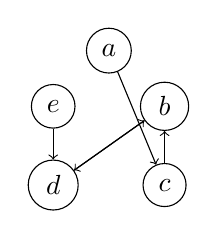
\begin{tikzpicture}[baseline=(e)]
\tikzstyle{state}=[shape=circle,draw,minimum size=0.4cm]

\node[state] (a) {$a$};
\node[state, below right of = a] (b) {$b$};
\node[state, below of = b] (c) {$c$};
\node[state, below left of = a](0,0) (e) {$e$};
\node[state, below of = e](0,0) (d) {$d$};

\path[->,draw] (a) edge (c);
\path[->,draw] (c) edge (b);
\path[->,draw] (b) edge (d);
\path[->,draw] (d) edge (b);
\path[->,draw] (e) edge (d);
\end{tikzpicture}
 \\ \midrule
% once printed, draw in G(P) from 6.1.c

Facts
& A type of rule: atoms stated in this way are unconditinoally true. (\texttt{a. b.} = \texttt{a :- . b :- .})
&& \texttt{a. \newline
	b. \newline
	---------- \newline
	\{ a, b \} } &\\ \midrule


Fitting Semantics $\Phi$
& A program's completion in the form of an operator (as such, Fitting Semantics results in supported models in the form of an interpretation, formatted like $\langle \{\top\}, \{\bot\} \rangle$) where the stuff in $\{\top\}$ is a supported model.
If the program is tight, i.e.\ there are no loops, then the stuff in $\{\top\}$ is also a stable model.
If the program is not tight, then Fitting Semantics can't be used to determine the stable model; need Wellfounded Semantics instead.
&& (walkthrough in \ref{subsec:fitting-sem}) &\\ \midrule


Interpretation
& An assignment of all atoms in a program to true and false.
&& -- &\\ \midrule

Interpretation, partial
& An assignment of some atoms in a program to true and false, written $\langle \{\top\}, \{\bot\} \rangle$, e.g.\ $\langle \{a\}, \{b\} \rangle$ means that $a$ is true and $b$ is false.
&& -- &\\ \midrule

Intervals
& Ranges of numbers are notated as follows: \texttt{start .. end}, where \texttt{end} $\geq$ \texttt{start}. 
Going in the other direction (i.e.\ starting with the larger value) returns no values.
&& \texttt{%
	a(1..3). \newline
	---------- \newline
	\{ a(1), a(2), a(3) \}} 
& \texttt{%
	a(3..1). \newline
	---------- \newline
	\{ \}}
\\ \midrule

Loops
& Two or more atoms that are defined in terms of each other. Can be easily identified by drawing a dependency graph.
If two loops have a node in common, then those two loops can also be joined into a larger loop.
A program can have multiple loops.
&& -- &\\ \midrule

Loops, even \newline through negation\slash \newline multiple paths \newline (Ex.\ 1 Part 1  1.4)
& Triggered by a particular mutually contradictory statement (at right), take different paths through the rules, assuming for the first path that, say, \texttt{a} is true and \texttt{b} is false, and for the next path, that \texttt{a} is false and \texttt{b} is true.
This can lead to multiple stable models.

&& Trigger: \newline
\texttt{%
	a :- not b. \newline
	b :- not a. \newline
	---------- \newline
	\{ a \} \newline
	\{ b \}}
& \texttt{%
	a :- not b. \newline
	b :- not a, d. \newline
	d. \newline
	----------- \newline
	\{ a, d \} \newline
	\{ b, d \}} \newline \\ %\midrule


& If there are multiple triggers, i.e.\ that mutually contradictory statement shows up once with, say, \texttt{a} and \texttt{b} and also once with \texttt{c} and \texttt{d}, then every combination of these has to be explored.
&& \texttt{%
	a :- not b. \newline
	b :- not a. \newline
	c :- not d. \newline
	d :- not c. \newline
	---------- \newline
	\{ a, c \} \newline
	\{ a, d \} \newline
	\{ b, c \} \newline
	\{ b, d \}}
&\\ \midrule

Loops, odd \newline through negation\slash \newline paradoxes \newline (Ex.\ 1 Part 1  1.5, 1.6)
& There is no way to resolve the statement \texttt{a :- not a.}, because if the body tells us one truth value for \texttt{a}, the head tells us the other.
So this statement produces no stable models, i.e.\ it is unsatisfiable.		
&& \texttt{%
	a :- not a. \newline
	---------- \newline}
\textit{[unsatisfiable]}
& \\ %\midrule

%	Paradoxes with \newline complex bodies \newline (Ex.\ 1 Part 1  1.5, 1.6)
& If the rest of the body is true, then we reach the paradox, meaning that the model is unsatisfiable (left).
If there is one false atom in the body, then the rule can no longer tell us anything about the head, so we avoid the paradox and can satisfy the program (right).
&& \texttt{%
	a :- not a, d. \newline
	d. \newline
	---------- \newline}
\textit{[unsatisfiable]}
& \texttt{%
	a :- not a, b. \newline
	b :- c. \newline
	---------- \newline
	\{ \} } \\ \midrule


Loop formulas $LF(P)$
& For atoms in a loop to be true, they need to have some kind of external support. i.e.\ be justifiable using a rule whose head contains a loop atom and whose 
So, loop formulas are used for identifying external support for loop atoms:\ they are the disjunctions of all bodies of rules (a) whose head contains a loop atom and (b) whose positive body does not contain any atoms from the loop (it's OK if the negative body contains loop atoms, those may be contained in loop formulas).
There is one loop formula per loop in the program.
They can also be calculated on unfounded sets.
&& (walkthrough for a program in \ref{subsec:lf}, for unfounded sets in \ref{subsec:lf-unf}) &\\ \midrule

Model
& A set is a model if it satisfies all rules of a program.
A rule is satisfied if only its head is in the set, or if the head and the entire body is in the set.
For example, given the program \texttt{a :- b, c, d.}:\newline
\begin{tabular}{ll}
	\texttt{ \{ c, d \} } & Not a model (does not satisfy body or head of rule)\\
	\texttt{ \{ b, c, d \} } & Not a model (satisfies body of rule but not head)\\
	\texttt{ \{ a, b, c, d \} } & A model (satisfies body and head of rule)\\			
\end{tabular}

Stable model (adds acyclic support) $\subseteq$ supported model (adds support) $\subseteq$ model
&& -- &\\ \midrule

Model, stable
& A set is a stable model (or ``answer set'') if it is a model (i.e.\ if it satisfies all the rules of a program) \textit{and} if there is justification in the program for every atom (i.e.\ if each atom is provably true).
The program \texttt{a :- b, c, d.} has no stable models, since none of the atoms are justified. 
There can be multiple stable models if there are multiple ``paths'' through a set of rules, e.g.\ as provoked by a choice rule (see below). 
You compute stable models using reducts (see below). \newline

\textit{Note:} Stable models are represented in what follows as atoms between \texttt{\{\}} below \texttt{-----} after all of the rules of the program.
&& \texttt{a. \newline
	---------- \newline
	\{ a \}} &\\ \midrule

Model, supported
& A supported model is one where the program offers support for every atom in the model.
We get supported models from the Clark's Completion of a program.
If a program is tight (i.e.\ there are no loops), then a supported model is a stable model.
If the program is not tight, then loop formulas are used to determine whether a supported model is a stable model (if the supported model satisfies the implication in the loop formula, then it is a stable model).
&& (walkthrough in \ref{subsec:compl-supp}) &\\ \midrule

Mutual definition \newline (Ex.\ 1 Part 1: 1.1)
& If two atoms are defined exclusively in terms of one another, both are considered false, since they cannot independently be proven true.
The empty set is the result because it is the minimal stable model (but it can be removed by constraints; see below).
&& \texttt{%
	a :- b. \newline
	b :- a. \newline
	---------- \newline				
	\{ \} } &\\ \midrule

Negation \newline (Ex.\ 1 Part 1: 1.2, 1.3)
& True if the contained atom is not true or not provable (see ``Truth'' above).
&& \texttt{a :- not b. \newline
	---------- \newline
	\{ a \} } 
& \texttt{a :- not b, c. \newline
	b :- not a, d. \newline
	c. \newline
	---------- \newline
	\{ a, c \}} \\ \midrule


Nogoods
& Sets of assignments of truth values to certain atoms that cannot all hold at the same time.
An atom that must be true is formatted like $\ngta{a}$, a body that must be true $\ngtb{a}$, an atom that must be false $\ngfa{a}$, and a body that must be false $\ngfb{a}$.

The set of $\Delta$ nogoods (completion nogoods) deals with the supported model. This set contains head and body nogoods and is based on the completion.
The set of $\delta$ nogoods (loop nogoods) is based on the loop formulas and ensures external support for atoms in loops.
Nogoods are used for conflict analysis and backjumping.
&& (walkthrough in \ref{subsec:ng}) &\\ \midrule

Optimisation: maximise, minimise \newline (Ex.\ 1 Part 2 1.5)
& Optimisation lets us choose between several stable models to find one that meets a particular condition. The \texttt{\#maximize} and \texttt{\#minimize} directives do the same thing as the \texttt{\#sum} directive above, but with one more step: they calculate the sums for all stable models and only let those models through into the final answer that have the largest (for \texttt{\#maximize}) or smallest (for \texttt{\#minimize}) sum. \newline

In the example, the second line generates the sets \texttt{\{a(1)\}}, \texttt{\{a(2)\}}, and \texttt{\{a(1), a(2)\}} (see set generators above).
The first two of those have a sum of 1, while the second has a sum of 2.
Because its sum is greater than the minimum of 1, \texttt{\{a(1), a(2)\}} is removed as a candidate by the \texttt{\#minimize} directive.

&& {\footnotesize\texttt{%
		b(1..2).\newline
		1 \{ a(X) : b(X) \}.\newline
		\#minimize\{ 1,X : a(X) \}.\newline
		\#show a/1.\newline
		---------- \newline
		\{ a(1) \} \newline
		\{ a(2) \} \newline
}} &\\  \midrule







Program
& Defined as a set of rules. A positive program contains only rules that contain no negation. A normal program contains at least one rule containing negation. &&&\\ \midrule

Python functions \newline (Ex.\ 1 Part 2 1.6)
& Between the \texttt{\#script(python)} and \texttt{\#end.} directives, you can define a Python function that returns some value.
When you call that function later in the ASP program (prefacing the function name with the at symbol), the value that the function returns is what will be used, say, as a value for a variable.

&& {\small\texttt{%
		\#script(python) \newline
		def value(): \newline
		\mbox{~~~~}return 1 \newline
		\#end. \newline \newline
		a(X) :- X = [AT]value(). \newline
		---------- \newline
		\{ a(1) \}
}} \\ \midrule

Reduct
& The reduct of a set $X$ is written as $P^x$ and is used to determine which models of a program are stable.
It makes a normal program $P$ positive, wrt a given set of atoms $X$.
Formally:
\begin{center}
	$P^X = \{h(r) \leftarrow B^+(r) | r \in P\ \text{such that}\ B^-(r) \cap X = \varnothing \}$
\end{center}
where $h$ = head of rule, $r$ = rule, $B^+(r)$ = atoms in body of rule that are positive (i.e.\ contain no negation), $B^-(r)$ = atoms in body of rule that are negative. \newline

What this says is that the reduct contains (a) no rules that have an atom in their negative body that is also in $X$ (these are removed because we know we can't use them to justify anything, since the atom is negative in the rule but positive in our set $X$) and (b) only the positive parts of rules that have a negative atom in their body whose positive counterpart isn't in $X$ (i.e.\ all negative atoms are removed).
You are left with a positive program $P^X$. \newline

&& (walkthrough in \ref{subsec:reduct}) &\\ \midrule

Reduct, consequence of
& The atoms that you can justify using the reduct $P^X$, i.e.\ the left-over positive program (see above), are the consequence of the reduct, written $Cn(P^X)$.
If $Cn(P^X) = X$, i.e.\ if what you put in is the same as what you get out, then you have yourself a stable model.
&& -- &\\ \midrule


Rules
& Consist of a head (to the left of the implication \texttt{:-}, the computer-readable version of $\leftarrow$) and a body (to the right of the implication) and ends with a period.
The head is true if the body is true.
If the body contains conjunctions, as soon as one conjunct is false, the rule cannot be used any more because it is not true. \newline

\textit{Note:} As soon as one rule shows an atom to be true, even if other rules do not, then that atom is always true. 
If a rule's body is false, it does not mean that the head is false -- it means we cannot use the rule to prove the head.
So even if we have conflicting results (i.e.\ one rule says an atom is true, another does not say it's true), then the atom is true.
&& \texttt{a :- b.} &\\ \midrule

Safety
&  A rule is safe if all variables appearing anywhere within it also appear in its positive body, or in the condition of a set generator. 
A program is safe if all rules are safe.
A program needs to be safe because an unsafe program means that there is no domain of the variables (i.e.\ no mapping of variables to atoms), and we need a domain in order to ground the program so it can be solved.
&& -- &\\ \midrule	

Set generators \newline (Ex.\ 1 Part 2 1.2)
& Generates candidate stable models using the following notation: \texttt{\{set contents : condition\}}, where numbers on either side indicate the required cardinality of the set (see cardinality rules above).
For example, given the facts \texttt{b(1). b(2).}, the set generator \texttt{\{ a(X) : b(X) \}.} generates the following four sets: \texttt{\{\}}, \texttt{\{a(1)\}}, \texttt{\{a(2)\}}, and \texttt{\{a(1), a(2)\}}.
The facts we know are also part of each model, so for example, the model formed by the set generator's second set is \texttt{\{ b(1), b(2), a(1) \}}. \newline

These can also be used in the heads of rules, as shown in the examples. 
Note that if there are facts of form \texttt{c(Y)} for multiple \texttt{Y}s, then the rule is applied for each candidate model as many times as there are \texttt{Y}s (right).

&& {\tiny\texttt{%
		b(1). b(2). c(3). \newline
		1 \{ a(X, Y) : b(X) \} 1 :- c(Y).\newline
		\#show a/2.\newline
		---------- \newline
		\{ a(2, 3) \} \newline
		\{ a(1, 3) \} \newline
}} &
{\tiny\texttt{%
		b(1). b(2). c(3). c(4). \newline
		1 \{ a(X, Y) : b(X) \} 1 :- c(Y).\newline
		\#show a/2.\newline
		---------- \newline
		\{ a(1, 3), a(1, 4) \} \newline
		\{ a(1, 3), a(2, 4) \} \newline
		\{ a(2, 3), a(1, 4) \} \newline
		\{ a(2, 3), a(2, 4) \} \newline
}}
\\ \midrule

Show statements \newline (Ex.\ 1 Part 2 1.6)
& Show statements can change the parts of the stable models that \textsc{clingo} displays.
Simply printing \texttt{\#show.} hides everything.
\texttt{\#show a/1.} shows only instances of the predicate \texttt{a} that has an arity (valence) of 1 (i.e.\ takes only one argument, e.g.\ \texttt{a(X)}).
\texttt{\#show a('yeah') : \#true.} is a conditional show directive that shows what's left of the colon if the condition on the right holds (as it does here; see Boolean literals above). 	
&& -- &\\ \midrule

Tightness
& If a program $P$ has no loops, then $P$ is said to be tight, and in those cases, a supported model of $P$ is also a stable model of $P$.
&& -- &\\ \midrule

Truth
& An atom is true if it can be proven by a fact or some other kind of rule, or if we assume it is as one path in a choice rule (see below).
If we do not know whether the atom is true or cannot prove that it is, we consider it to be false (closed world assumption). 
&& -- &\\ \midrule

Unfounded sets
& A set of atoms $U$ is unfounded wrt some partial interpretation if all of the rules whose heads are atoms in $U$ meet at least one of the following conditions:
\begin{itemize}[noitemsep]
	\item one atom of the rule's positive body is false in the partial interpretation (i.e.\  $\langle \{\}, \{\text{atom}\} \rangle$)
	\item one atom of the rule's negative body is true in the partial interpretation (i.e.\  $\langle \{\text{atom}\}, \{\} \rangle$)
	\item one atom of the rule's positive body is also in $U$
\end{itemize}

The easiest way to find unfounded sets is to first find the greatest unfounded set (GUS) and then check every subset in the GUS' power set for unfoundedness, using the above conditions.

Also, $\varnothing$ is by definition an unfounded set.
&& (walkthrough in \ref{subsec:unf}) &\\ \midrule

Unfounded set, greatest
& aka GUS. The union of all unfounded sets.
Computed by subtracting the minimal model of the program's reduct wrt some partial interpretation from the set of all atoms.
&& (walkthrough in \ref{subsec:unf})  &\\ \midrule


Unit propagation
& Recall that a nogood says that it cannot be the case that all of its elements (all of the truth conditions) hold.
Therefore, during conflict analysis, if all but one conditions of a nogood are fulfilled by a model (e.g.\ given the nogood $\{\ngta{a}, \ngfb{b}\}$, if we  know that $\ngfb{b}$ but we don't know whether $a$ is true or false), then we must assume the opposite of what the remaining condition tells us (e.g.\ we must assume $\ngfa{a}$), since it cannot be the case that both $\ngta{a}, \ngfb{b}$ hold. We already know that $\ngfb{b}$ holds, so the other one cannot hold.
&& (walkthrough in \ref{subsec:ng-confl}) &\\ \midrule

Wellfounded Semantics $\Omega$
& Uses the greatest unfounded set to determine the stable model of a program by identifying the atoms that are acyclically supportable in a program and (the important ability) identifying the atoms that are not acyclically supportable, including those in loops. 
Also in the form of $\langle \{\top\}, \{\bot\} \rangle$, where $\{\top\}$ is a stable model and $\{\bot\}$ is the set of atoms that are not acyclically derivable.
&& (walkthrough in \ref{subsec:wellf-sem}) &\\
\end{longtable}


\pagebreak


% ----------------------------------------------------------------------

\section{Answers to the quiz questions}

\begin{itemize}
	
	\item[2] \textbf{Positive programs and stable models}
	\begin{itemize}[noitemsep]
		\item If a positive rule is satisfied by a set of (ground) atoms, then it is not true that each of its supersets satisfies the rule as well.
		\begin{itemize}[noitemsep]
			\item Because $\varnothing$ satisfies a positive rule like $a \leftarrow b$, but $\{b\}$ is a superset of $\varnothing$ and does not satisfy this rule (would need $\{b, a\}$).
		\end{itemize}
		\item Each positive logic program has some model.
		\item Each positive logic program has some stable model.
		\item A positive rule with variables is not necessarily satisfied by a set of (ground) atoms if some ground instance of the rule is satisfied by the set of atoms (all ground instances of the rule have to be satisfied, not just one).
		\item The stable model of a positive logic program is contained in each model of the logic program (because a SM is the minimal requirement for a set to be a model).
	\end{itemize}
	
	\item[3] \textbf{Normal logic programs, stable models, reducts}
	\begin{itemize}[noitemsep]
		\item Each normal logic program has some model.
		\item However, each normal logic program does not necessarily have a stable model.
		\item Given a normal logic program $P$, it is not true that the reduct $P^X$ is contained in $P^Y$ for each subset $X$ of a set of $Y$ atoms.
		\begin{itemize}[noitemsep]
			\item Because the reduct gets smaller if there are more atoms, since more rules get crossed out. So $X$ being a subset of $Y$ (i.e.\ $Y$ has more atoms, is more restrictive) means that the reduct $P^Y$ is a subset of the reduct $P^X$, rather than the other way around.
		\end{itemize}
		\item If a set $X$ of atoms is a model of a normal logic program $P$, then $X$ is a model of the reduct $P^Y$ for each superset $Y$ of $X$.
		\item Given a normal logic program $P$, each stable model of $P$ is a proper subset minimal model of $P$.
	\end{itemize}
	
	\item[4] \textbf{Choice rules and integrity constraints}
	\begin{itemize}[noitemsep]
		\item Each interpretation (combination of atoms) satisfies a choice rule without lower and upper bounds, i.e.\ $0 \{ \ldots \} \infty$.
		\item It is not true that a logic program without choice rules has at most one stable model.
		\begin{itemize}[noitemsep]
			\item If a logic program has even loops through negation, then there can be two stable models, since $1\{a, b\}1$ is the same as $\{a \leftarrow {\sim} b, b \leftarrow {\sim} a\}$.
		\end{itemize} 
		\item The stable models of a logic program $P \cup C$, where $C$ is a set of integrity constraints, are stable models of $P$.
		\begin{itemize}[noitemsep]
			\item Constraints can only remove answer sets / prune them, not change whether or not something is a stable model or not.
		\end{itemize}
		\item A logic program without integrity constraints does not necessarily have a stable model.
		\begin{itemize}[noitemsep]
			\item For example, if there is an odd loop (a.k.a.\ a paradox), like $a \leftarrow not a$ -- this can result in no SM without there being an integrity constraint.
		\end{itemize}
		\item ASP systems do not first evaluate choice rules and then prune stable model candidates that violate integrity constraints.
	\end{itemize}
	
	\item[5] \textbf{Safety, grounding}
	\begin{itemize}[noitemsep]
		\item It is not true that a rule is safe if all variables in its head also appear in its body. It should be: A rule is safe if all variables anywhere within it also appear in its positive body.
		\begin{itemize}[noitemsep]
			\item Example of unsafe rule: $a(X) \leftarrow {\sim} b(X)$. $X$ does not appear in a positive body.
		\end{itemize}
		\item It is not true that each safe program has a finite number of finite stable models.
		\begin{itemize}[noitemsep]
			\item Example of a program that is safe but that gives an infinite SM: $\{ P(X+1) \leftarrow P(X). P(0). \}$ gives $\{0, 1, 2, 3, \ldots, \infty \}$.
		\end{itemize}
		\item It is not true that grounders (partially) evaluate the body literals of a rule in the order given by an encoding. Order of literals in body doesn't matter for grounder.
	\end{itemize}
	
	\pagebreak
	
	\item[6] \textbf{Clark's Completion and loop formulas}
	\begin{itemize}[noitemsep]
		\item It is not true that, if a set of atoms $X$ is a model of a normal program $P$, then $X$ is a model of $CF(P)$.
		\begin{itemize}[noitemsep]
			\item Example: The set $X = \{a\}$ is a model of $P = \{a \leftarrow {\sim} a\}$, but not of  $CF(P) = \{a \leftrightarrow \neg a\}$
		\end{itemize}
		\item Given a normal program $P$, if a set of atoms $X$ is a model of $CF(P)$, then $X$ is a model of $P$.
		\item Given a normal program $P$, it is not true that, if a set of atom $X$ is a model of $CF(P)$, then $X$ is a stable model of $P$.
		\begin{itemize}[noitemsep]
			\item Example: Given the program $P = \{a \leftarrow a\}$, $X = \{a\}$ is a model of the completion but not a stable model.
		\end{itemize}
		\item If $X$ is a stable model of a normal program $P$, then $X$ is a model of $CF(P)$.
		\item Given a normal program $P$, it is not true that, if $CF(P)$ has (at least) one model, then $P$ has (at least) one stable model.
		\begin{itemize}[noitemsep]
			\item Example: For the program $P = \{a \leftarrow a, a \leftarrow {\sim} a\}$, $X = \{a\}$ is a model of the completion $CF(P) = \{a \leftrightarrow (a \lor \neg a)\}$, but $P$ has no stable models.
		\end{itemize}
		\item Let $P$ be a normal program and $L_1, L_2 \in loop(P)$. If $(L_1 \cap L_2) \neq \varnothing$, then $(L_1 \cup L_2) \in loop(P)$.
	\end{itemize}
	
	\item[8] \textbf{Nogoods, conflict-driven ASP solving}
	\begin{itemize}[noitemsep]
		\item It is not the case that, to compute the stable models of a logic program $P$, ASP systems first construct a flat internal representation of the completion nogoods and the loop nogoods in $\Delta_P \cup \Lambda_P$ (in the notation of the printed exercises---for this document, this corresponds to  $\Delta_P \cup \delta_P$, which I use because this notation was used in the tutorials).
		\item For each tight logic program, the solutions of $\Delta_P$ coincide with the solutions of $\Delta_P \cup \Lambda_P$ (again, $\Delta_P \cup \delta_P$ here).
		\item A Unique Implication Point (UIP) of a decision level, along with literals assigned at smaller decision levels, lead to a conflict by propagation.
		\item Each decision level beyond 0 at which a conflict occurs has some UIP.
		\item If a logic program has no stable model, it is false that conflict-driven ASP solving procedures may loop infinitely.
	\end{itemize}
\end{itemize}

% ----------------------------------------------------------------------

\vfill \hfill This version compiled on \today.

}
	
\end{document}